\documentclass[11pt,a4paper]{article}
\usepackage[spanish,es-nodecimaldot]{babel}
\usepackage[utf8]{inputenc}
\usepackage[T1]{fontenc}
\usepackage{lmodern}
\usepackage[top=1.8cm,bottom=1.8cm,left=2.0cm,right=2.0cm,headheight=15pt]{geometry}
\usepackage{amsmath,amssymb}
\usepackage[table]{xcolor}
\usepackage{booktabs,tabularx,array}
\usepackage[most]{tcolorbox}
\usepackage{graphicx}
\usepackage{float}
\usepackage{caption}
\usepackage{tikz}
\usetikzlibrary{arrows.meta,positioning,shapes.geometric,calc}
\usepackage{enumitem}
\usepackage{fancyhdr}
\usepackage{hyperref}
\usepackage{microtype}
\usepackage{ragged2e}
\usepackage{lscape}

\definecolor{azul}{HTML}{24557A}
\definecolor{azulclaro}{HTML}{EAF3F9}
\definecolor{verde}{HTML}{277A54}
\definecolor{verdeclaro}{HTML}{EAF6EF}
\definecolor{naranja}{HTML}{C46A1B}
\definecolor{naranjaclaro}{HTML}{FFF3DD}
\definecolor{rojo}{HTML}{B33B3B}
\definecolor{rojoclaro}{HTML}{FBEAEA}
\definecolor{gris}{HTML}{4E5962}
\definecolor{grisclaro}{HTML}{F2F4F5}
\definecolor{morado}{HTML}{654A86}
\definecolor{moradoclaro}{HTML}{F2EDF8}

\hypersetup{colorlinks=true,linkcolor=azul,urlcolor=azul,pdftitle={Estadística 2 - Unidad 2: Pruebas de hipótesis}}
\setlength{\parindent}{0pt}
\setlength{\parskip}{5pt plus 1pt minus 1pt}
\linespread{1.025}
\setlist[itemize]{leftmargin=1.5em,itemsep=3pt,topsep=4pt,
  label=\textcolor{azul}{\small\textbullet}}
\setlist[enumerate]{leftmargin=1.7em,itemsep=3pt,topsep=4pt,
  label=\textcolor{azul}{\bfseries\arabic*.}}
\renewcommand{\arraystretch}{1.2}
\setlength{\emergencystretch}{2em}

\pagestyle{fancy}
\fancyhf{}
\fancyfoot[C]{\textcolor{gris}{\thepage}}
\renewcommand{\headrulewidth}{0pt}

\newcolumntype{Y}{>{\RaggedRight\arraybackslash}X}
\newcolumntype{C}[1]{>{\Centering\arraybackslash}p{#1}}
\newcolumntype{L}[1]{>{\RaggedRight\arraybackslash}p{#1}}
\newcommand{\Hcero}{H_0}
\newcommand{\Huno}{H_1}
\newcommand{\EE}{\operatorname{EE}}
\newlength{\subcontentwidth}
\setlength{\subcontentwidth}{\textwidth}
\newsavebox{\studybox}

\newenvironment{regla}[1][Regla para recordar]{%
  \par\medskip\noindent\begingroup\setlength{\fboxsep}{7pt}%
  \begin{lrbox}{\studybox}\begin{minipage}{\dimexpr\linewidth-2\fboxsep\relax}
  \color{verde}\textbf{#1}\par\smallskip\color{black}}{%
  \par\end{minipage}\end{lrbox}\colorbox{verdeclaro}{\usebox{\studybox}}\endgroup\par\medskip}
\newenvironment{idea}[1][Idea clave]{%
  \par\medskip\noindent\begingroup\setlength{\fboxsep}{7pt}%
  \begin{lrbox}{\studybox}\begin{minipage}{\dimexpr\linewidth-2\fboxsep\relax}
  \color{azul}\textbf{#1}\par\smallskip\color{black}}{%
  \par\end{minipage}\end{lrbox}\colorbox{azulclaro}{\usebox{\studybox}}\endgroup\par\medskip}
\newenvironment{advertencia}[1][Atención]{%
  \par\medskip\noindent\begingroup\setlength{\fboxsep}{7pt}%
  \begin{lrbox}{\studybox}\begin{minipage}{\dimexpr\linewidth-2\fboxsep\relax}
  \color{naranja}\textbf{#1}\par\smallskip\color{black}}{%
  \par\end{minipage}\end{lrbox}\colorbox{naranjaclaro}{\usebox{\studybox}}\endgroup\par\medskip}
\newenvironment{conclusion}[1][Conclusión]{%
  \par\medskip\noindent\begingroup\setlength{\fboxsep}{7pt}%
  \begin{lrbox}{\studybox}\begin{minipage}{\dimexpr\linewidth-2\fboxsep\relax}
  \color{gris}\textbf{#1}\par\smallskip\color{black}}{%
  \par\end{minipage}\end{lrbox}\colorbox{grisclaro}{\usebox{\studybox}}\endgroup\par\medskip}
\newenvironment{programa}[1][Uso de R]{%
  \par\medskip\noindent\begingroup\setlength{\fboxsep}{7pt}%
  \begin{lrbox}{\studybox}\begin{minipage}{\dimexpr\linewidth-2\fboxsep\relax}
  \color{morado}\textbf{#1}\par\smallskip\color{black}}{%
  \par\end{minipage}\end{lrbox}\colorbox{moradoclaro}{\usebox{\studybox}}\endgroup\par\medskip}
\tcbset{
  rcheat/.style={
    enhanced, colback=white, colframe=morado!55!black,
    colbacktitle=morado!82!black, coltitle=white,
    fonttitle=\small\bfseries, boxrule=.4pt, arc=1.2mm,
    top=2mm, bottom=2mm, left=3mm, right=3mm,
    toptitle=1mm, bottomtitle=1mm,
    before skip=1mm, after skip=1mm
  },
  rscript/.style={
    enhanced, colback=gray!8, colframe=gray!45,
    boxrule=.3pt, arc=.7mm,
    top=1mm, bottom=1mm, left=1.5mm, right=1.5mm,
    before skip=.8mm, after skip=.8mm,
    fontupper=\ttfamily\scriptsize
  },
  rverdict/.style={
    enhanced, colback=moradoclaro, colframe=moradoclaro,
    boxrule=0pt, borderline west={1.2pt}{0pt}{morado},
    arc=.5mm, top=.8mm, bottom=.8mm, left=2mm, right=1mm,
    before skip=.8mm, after skip=0mm,
    fontupper=\small
  }
}
\newtcolorbox{rcheat}[1]{rcheat,title={#1}}
\newtcolorbox{rscript}{rscript}
\newtcolorbox{rverdict}{rverdict}
\newcommand{\rsubentry}[1]{%
  \refstepcounter{subsection}%
  \phantomsection\addcontentsline{toc}{subsection}{\protect\numberline{\thesubsection}#1}}
\newcommand{\rsubhead}[1]{%
  \rsubentry{#1}%
  \par\noindent{\color{morado}\small\bfseries \thesubsection\quad #1}\par\vspace{.5mm}}

\tikzset{
  decision/.style={draw=naranja,very thick,diamond,aspect=2.2,fill=naranjaclaro,
    align=center,text width=3.2cm,font=\small\bfseries,inner sep=1mm},
  result/.style={draw=azul,thick,rounded corners=2mm,fill=azulclaro,
    align=center,text width=4.2cm,font=\small,inner sep=2mm},
  treeq/.style={draw=naranja,very thick,diamond,aspect=2.2,fill=naranjaclaro,
    align=center,text width=3.3cm,font=\small\bfseries,inner sep=1mm},
  treeout/.style={draw=azul,thick,rounded corners=2mm,fill=azulclaro,
    align=center,text width=3.0cm,minimum height=2.25cm,font=\small,inner sep=1.6mm},
  treewarn/.style={treeout,draw=naranja,fill=naranjaclaro},
  treelargeq/.style={draw=naranja,very thick,diamond,aspect=2.35,fill=naranjaclaro,
    align=center,text width=4.6cm,font=\normalsize\bfseries,inner sep=2mm},
  treelargeout/.style={draw=azul,very thick,rounded corners=2mm,fill=azulclaro,
    align=center,text width=5.0cm,minimum height=3.0cm,font=\normalsize,inner sep=2.5mm},
  treelargewarn/.style={treelargeout,draw=naranja,fill=naranjaclaro},
  onemeanq/.style={draw=naranja,thick,diamond,aspect=2.05,fill=naranjaclaro,
    align=center,text width=2.8cm,font=\scriptsize\bfseries,inner sep=.8mm},
  onemeanout/.style={draw=azul,thick,rounded corners=1.5mm,fill=azulclaro,
    align=center,text width=2.55cm,minimum height=2.55cm,font=\scriptsize,inner sep=1.1mm},
  onemeanwarn/.style={onemeanout,draw=naranja,fill=naranjaclaro},
  arrow/.style={-{Latex[length=2mm]},thick,draw=gris},
  edgeword/.style={fill=white,inner sep=1pt,font=\small\bfseries}
}

% Jerarquía visual: las secciones vuelven al margen; los subtítulos y su contenido
% quedan subordinados mediante una sangría estable.
\makeatletter
\renewcommand\section{\par\global\leftskip=0pt
  \@startsection{section}{1}{0pt}{3.6ex plus 1ex minus .2ex}{1.6ex}
  {\normalfont\Large\bfseries\color{azul}}}
\renewcommand\subsection{\par\global\leftskip=0pt
  \@startsection{subsection}{2}{0pt}{2.8ex plus .8ex minus .2ex}{1.1ex}
  {\normalfont\large\bfseries\color{gris}}}
\makeatother

\begin{document}
\hypersetup{pageanchor=false}

\begin{titlepage}
\thispagestyle{empty}
\centering
\vspace*{1.8cm}
{\color{azul}\rule{\textwidth}{1.2pt}}\\[1.2cm]
{\fontsize{29}{34}\selectfont\bfseries\color{azul} Estadística 2}\\[5mm]
{\LARGE Unidad 2: Pruebas de hipótesis}\\[1.2cm]
\fcolorbox{azul}{grisclaro}{\begin{minipage}{.78\textwidth}\RaggedRight
\textbf{\color{azul}Tema A: Hipótesis}
\begin{itemize}[leftmargin=1.4em,itemsep=2pt,topsep=3pt]
\item Hipótesis nula y prueba de significancia.
\item Hipótesis relativas a una media.
\end{itemize}
\medskip
\textbf{\color{azul}Tema B: Características de operación}
\begin{itemize}[leftmargin=1.4em,itemsep=2pt,topsep=3pt]
\item Curvas características de operación.
\item Trazado de las curvas.
\item Hipótesis relativas a dos medias.
\end{itemize}
\end{minipage}}
\vfill
{\color{azul}\rule{\textwidth}{1.2pt}}
\end{titlepage}

\hypersetup{pageanchor=true}
\pagenumbering{roman}
\tableofcontents
\clearpage
\pagenumbering{arabic}

% =============================================================================
\section{Conceptos fundamentales}

\subsection{Hipótesis y prueba de hipótesis}

\textbf{Hipótesis.} Es una suposición sobre un parámetro de la población que debe verificarse mediante evidencia muestral.

\textbf{Prueba de hipótesis.} Es un procedimiento estandarizado para decidir si la evidencia disponible permite rechazar una afirmación acerca de un parámetro poblacional.

\textbf{Hipótesis nula ($\Hcero$).} Es el punto de partida y se asume temporalmente para confrontarla con los datos. Contiene la igualdad: $=$, $\le$ o $\ge$.

\textbf{Hipótesis alternativa ($H_a$ o $\Huno$).} Expresa lo que se concluirá si existe evidencia suficiente para rechazar $\Hcero$. Se formula con $<$, $>$ o $\ne$.

\begin{regla}
El signo de $\Huno$ funciona como una flecha hacia la región de rechazo:
\[
\Huno:\mu>\mu_0\Rightarrow\text{cola derecha},\qquad
\Huno:\mu<\mu_0\Rightarrow\text{cola izquierda},
\]
\[
\Huno:\mu\ne\mu_0\Rightarrow\text{prueba bilateral o de dos colas}.
\]
\end{regla}

\begin{center}
\begin{tikzpicture}[node distance=12mm]
\node[decision] (d) {¿Qué signo tiene $\Huno$?};
\node[result,below left=17mm and 25mm of d] (r) {$\Huno:\mu>\mu_0$\\cola derecha\\rechazar si $z>z_\alpha$};
\node[result,below=17mm of d] (l) {$\Huno:\mu<\mu_0$\\cola izquierda\\rechazar si $z<-z_\alpha$};
\node[result,below right=17mm and 25mm of d] (b) {$\Huno:\mu\ne\mu_0$\\dos colas\\rechazar si $|z|>z_{\alpha/2}$};
\draw[arrow] (d)--node[edgeword,above left]{$>$}(r);
\draw[arrow] (d)--node[edgeword,right]{$<$}(l);
\draw[arrow] (d)--node[edgeword,above right]{$\ne$}(b);
\end{tikzpicture}
\end{center}

\subsection{Nivel de significancia}

El nivel de significancia determina qué tan extrema debe ser la evidencia para rechazar $\Hcero$.
Los valores más usuales son $\alpha=0.05$ y $\alpha=0.01$. En una prueba bilateral, el nivel total se divide en $\alpha/2$ en cada cola.

\begin{idea}
Antes de calcular debe decidirse: qué parámetro se estudia, qué quiere demostrar el problema, qué cola corresponde, qué valor de $\alpha$ se usará y con qué distribución se trabajará.
\end{idea}

% =============================================================================
\section{Procedimiento para una prueba de hipótesis}

Cada ejercicio sigue la misma secuencia:

\begin{enumerate}[label=\textbf{Paso \arabic*.},wide=0pt,leftmargin=0pt,labelsep=.55em]
\item Preguntar qué quiere demostrar el problema.
\item Formular $\Hcero$ y $\Huno$.
\item Mirar el signo de $\Huno$ y determinar si la prueba es derecha, izquierda o bilateral.
\item Fijar el nivel de significancia $\alpha$.
\item Elegir el estadístico: $Z$, $t$, $Z_{\bar X_1-\bar X_2}$, $t_{\bar X_1-\bar X_2}$ u otro que corresponda.
\item Encontrar el valor crítico y construir la región de rechazo.
\item Calcular $z_{calc}$ o $t_{calc}$ con los datos de la muestra.
\item Comparar el estadístico calculado con el valor crítico, o comparar el $p$-valor con $\alpha$.
\item Decidir: rechazar $\Hcero$ o no rechazar $\Hcero$.
\item Interpretar la decisión con las palabras del problema.
\end{enumerate}

\begin{conclusion}
Una conclusión correcta no termina en ``se rechaza'' o ``no se rechaza''. Debe expresar qué significa la decisión para la población y el problema estudiado.
\end{conclusion}

% =============================================================================
\section{Elección de la distribución y del estadístico}

\subsection{\texorpdfstring{Una media: estadísticos $Z$ y $t$}{Una media: estadísticos Z y t}}

Para una media, las dos formas principales son:
\[
z_{calc}=\frac{\bar x-\mu_0}{\sigma/\sqrt n},
\qquad
t_{calc}=\frac{\bar x-\mu_0}{s/\sqrt n},
\qquad \nu=n-1.
\]

\begin{idea}[Cómo leer las fórmulas de una media]
El cociente compara la distancia entre la media observada y la media propuesta con el error estándar. Por eso, $z_{calc}$ o $t_{calc}$ indican a cuántos errores estándar se encuentra la muestra de $\mu_0$.
\smallskip
\small
\begin{tabularx}{\linewidth}{@{}YY@{}}
$\bar x$: media calculada con la muestra. & $\mu_0$: media poblacional propuesta en $\Hcero$.\\[2pt]
$\sigma$: desviación poblacional conocida; $s$: desviación muestral que la estima. & $n$: tamaño muestral; $\sigma/\sqrt n$ o $s/\sqrt n$: error estándar.\\[2pt]
$z_{calc}$ y $t_{calc}$: estadísticos calculados que se comparan con el valor crítico. & $\nu=n-1$: grados de libertad; $\alpha$: significancia; $z_\alpha$ y $z_{\alpha/2}$: valores críticos normales.
\end{tabularx}
\end{idea}

\begin{table}[H]
\centering
\caption{Selección del procedimiento según población, tamaño y conocimiento de $\sigma$.}
\small
\begin{tabularx}{\subcontentwidth}{L{3.1cm}L{3.2cm}YY}
\toprule
\rowcolor{azulclaro}
\textbf{Población} & \textbf{Tamaño de muestra} & \textbf{$\sigma$ conocida} & \textbf{$\sigma$ desconocida}\\
\midrule
\rowcolor{white}
Normal & Grande, $n\ge30$ & $Z$: usar $\sigma/\sqrt n$ & Según el criterio de la cátedra, $Z$ con $s/\sqrt n$\\
\rowcolor{grisclaro}
Normal & Pequeña, $n<30$ & $Z$: usar $\sigma/\sqrt n$ & $t$ de Student con $s/\sqrt n$ y $\nu=n-1$\\
\rowcolor{white}
No normal & Grande, $n\ge30$ & Aproximación $Z$ por TCL & Aproximación $Z$ con $s$ por TCL\\
\rowcolor{grisclaro}
No normal & Pequeña, $n<30$ & No aplicar automáticamente $Z$; el apunte original menciona cotas de Chebyshev & No aplicar automáticamente $t$; revisar otro método\\
\bottomrule
\end{tabularx}
\end{table}

\clearpage
\begin{landscape}
\pdfpageattr{/Rotate 90}
\thispagestyle{empty}
\subsection{Árbol de decisión completo para una media}

Comenzar por la forma de la población; después revisar el tamaño muestral y, por último, si $\sigma$ poblacional es conocida.

\begin{center}
\begin{tikzpicture}[x=1cm,y=1cm]
\node[onemeanq] (normal) at (0,0) {¿La población es aproximadamente normal?};

\node[onemeanq] (nN) at (-6.2,-2.25) {¿La muestra es grande?\\$n\ge30$};
\node[onemeanq] (nX) at (6.2,-2.25) {¿La muestra es grande?\\$n\ge30$};

\node[onemeanq] (sNG) at (-9.2,-4.65) {¿$\sigma$ poblacional conocida?};
\node[onemeanq] (sNP) at (-3.1,-4.65) {¿$\sigma$ poblacional conocida?};
\node[onemeanq] (sXG) at (3.1,-4.65) {¿$\sigma$ poblacional conocida?};
\node[onemeanq] (sXP) at (9.2,-4.65) {¿$\sigma$ poblacional conocida?};

\node[onemeanout] (a1) at (-10.7,-8.0) {\textbf{$Z$ de una media}\\[.6mm]
$\displaystyle z=\frac{\bar x-\mu_0}{\sigma/\sqrt n}$\\[.6mm]
Normal; $n\ge30$; $\sigma$ conocida.};
\node[onemeanout] (a2) at (-7.65,-8.0) {\textbf{$Z$ con $s$}\\[.6mm]
$\displaystyle z=\frac{\bar x-\mu_0}{s/\sqrt n}$\\[.6mm]
Criterio de la cátedra para muestra grande.};
\node[onemeanout] (a3) at (-4.6,-8.0) {\textbf{$Z$ de una media}\\[.6mm]
$\displaystyle z=\frac{\bar x-\mu_0}{\sigma/\sqrt n}$\\[.6mm]
Normal; $n<30$; $\sigma$ conocida.};
\node[onemeanout] (a4) at (-1.55,-8.0) {\textbf{$t$ de Student}\\[.6mm]
$\displaystyle t=\frac{\bar x-\mu_0}{s/\sqrt n}$\\[.6mm]
$\nu=n-1$; normal; $n<30$.};

\node[onemeanout] (a5) at (1.55,-8.0) {\textbf{$Z$ por TCL}\\[.6mm]
$\displaystyle z=\frac{\bar x-\mu_0}{\sigma/\sqrt n}$\\[.6mm]
No normal; $n\ge30$; $\sigma$ conocida.};
\node[onemeanout] (a6) at (4.6,-8.0) {\textbf{$Z$ con $s$ por TCL}\\[.6mm]
$\displaystyle z=\frac{\bar x-\mu_0}{s/\sqrt n}$\\[.6mm]
No normal; muestra grande.};
\node[onemeanwarn] (a7) at (7.65,-8.0) {\textbf{Cota de Chebyshev}\\[.6mm]
$\displaystyle \bar x\pm k\frac{\sigma}{\sqrt n}$\\[.6mm]
Cobertura mínima $1-1/k^2$; no es una prueba $Z$.};
\node[onemeanwarn] (a8) at (10.7,-8.0) {\textbf{No usar $t$ automáticamente}\\[.6mm]
$\bar x\pm k\,s/\sqrt n$ es solo una guía estimada.\\[.6mm]
Revisar otro método.};

\draw[arrow] (normal)--node[edgeword,above left]{sí}(nN);
\draw[arrow] (normal)--node[edgeword,above right]{no}(nX);
\draw[arrow] (nN)--node[edgeword,above left]{sí}(sNG);
\draw[arrow] (nN)--node[edgeword,above right]{no}(sNP);
\draw[arrow] (nX)--node[edgeword,above left]{sí}(sXG);
\draw[arrow] (nX)--node[edgeword,above right]{no}(sXP);
\draw[arrow] (sNG)--node[edgeword,above left]{sí}(a1);
\draw[arrow] (sNG)--node[edgeword,above right]{no}(a2);
\draw[arrow] (sNP)--node[edgeword,above left]{sí}(a3);
\draw[arrow] (sNP)--node[edgeword,above right]{no}(a4);
\draw[arrow] (sXG)--node[edgeword,above left]{sí}(a5);
\draw[arrow] (sXG)--node[edgeword,above right]{no}(a6);
\draw[arrow] (sXP)--node[edgeword,above left]{sí}(a7);
\draw[arrow] (sXP)--node[edgeword,above right]{no}(a8);
\end{tikzpicture}
\end{center}

\begin{idea}[Lectura rápida del árbol completo]
Con $\sigma$ conocida, el denominador usa $\sigma/\sqrt n$; si es desconocida, usa $s/\sqrt n$. Con muestra grande se trabaja con $Z$ según la guía. Con muestra pequeña, $t$ requiere población normal; si la población no es normal, no debe aplicarse automáticamente.
\end{idea}

\vfill
\hfill\textcolor{gris}{\thepage}
\end{landscape}
\pdfpageattr{}

\begin{advertencia}
El teorema de Chebyshev permite construir cotas del tipo $\bar x\pm k\sigma_{\bar X}$ con cobertura mínima $1-1/k^2$, pero no reemplaza sin más una prueba paramétrica normal. Para muestras pequeñas no normales debe revisarse el método apropiado.
\end{advertencia}

% =============================================================================
\section{Límites críticos: escala estandarizada y escala real}

Los dos métodos siguientes son equivalentes y llevan a la misma decisión.

\subsection{Método A: estadístico estandarizado}

Se transforma el promedio muestral en un puntaje estándar:
\[
z_{calc}=\frac{\bar x-\mu_0}{\sigma/\sqrt n}.
\]
Después se compara $z_{calc}$ con las abscisas críticas estándar. Por ejemplo, en una prueba bilateral con $\alpha=0.05$, los límites son aproximadamente $\pm1.96$.

\textbf{R, comando esencial:} \texttt{qnorm(1-alpha)} da el crítico derecho, \texttt{qnorm(alpha)} el izquierdo y \texttt{qnorm(1-alpha/2)} el crítico positivo bilateral. La explicación completa se encuentra en el anexo ``Resolución con R''.

\subsection{Método B: límites en unidades reales}

Se conserva $\bar x$ en sus unidades originales y se trasladan los valores críticos a la escala del problema. Para una prueba bilateral:
\[
LI=\mu_0-z_{\alpha/2}\frac{\sigma}{\sqrt n},
\qquad
LS=\mu_0+z_{\alpha/2}\frac{\sigma}{\sqrt n}.
\]
Para una prueba unilateral se utiliza solamente el límite del lado de rechazo:
\[
\text{derecha: }LS=\mu_0+z_\alpha\frac{\sigma}{\sqrt n},
\qquad
\text{izquierda: }LI=\mu_0-z_\alpha\frac{\sigma}{\sqrt n}.
\]

\textbf{R, comando esencial:} \texttt{qnorm()} también permite obtener el límite en unidades reales indicando $\mu_0$ como media y $\sigma/\sqrt n$ como desviación estándar. El código se reúne en el anexo.

% =============================================================================
\section{Errores tipo I y II}

\begin{table}[H]
\centering
\caption{Decisión tomada y realidad poblacional.}
\begin{tabular}{lcc}
\toprule
\rowcolor{azulclaro}
& \textbf{$\Hcero$ verdadera} & \textbf{$\Hcero$ falsa}\\
\midrule
\textbf{Rechazar $\Hcero$} & \cellcolor{rojoclaro}Error Tipo I: $\alpha$ & \cellcolor{verdeclaro}Decisión correcta: potencia $1-\beta$\\
\textbf{No rechazar $\Hcero$} & \cellcolor{verdeclaro}Decisión correcta: $1-\alpha$ & \cellcolor{naranjaclaro}Error Tipo II: $\beta$\\
\bottomrule
\end{tabular}
\end{table}

\begin{advertencia}[Interpretación correcta]
El \textbf{Error Tipo I} ocurre cuando se rechaza $\Hcero$ aunque sea verdadera. El \textbf{Error Tipo II} ocurre cuando no se rechaza $\Hcero$ aunque sea falsa. Si la decisión coincide con la realidad poblacional, no se comete ninguno de estos errores.
\end{advertencia}

% =============================================================================
\section{Curvas características de operación}

\begin{idea}[Cómo leer los símbolos de los gráficos]
\begin{itemize}
\item $\mu_0$: media establecida por la hipótesis nula; $\mu_1$: media alternativa que se desea detectar.
\item $\alpha$: riesgo de rechazar una hipótesis nula verdadera; $\beta$: riesgo de no detectar una alternativa real.
\item $1-\beta$: potencia de la prueba, es decir, su capacidad para detectar la alternativa.
\item $A$: frontera o valor crítico que separa la región de rechazo de la región de no rechazo.
\item Las áreas coloreadas representan probabilidades bajo las distribuciones correspondientes.
\end{itemize}
\end{idea}

\subsection{Prueba de cola derecha}

Con una región de rechazo a la derecha:
\begin{itemize}
\item cuando $\mu_1$ se desplaza hacia la derecha y se aleja de $\mu_0$, $\beta$ disminuye y la potencia aumenta;
\item cuando $\mu_1$ se desplaza hacia la izquierda y se acerca a la frontera desde la alternativa, $\beta$ aumenta.
\end{itemize}

\textbf{R, comando esencial:} \texttt{dnorm(x, mean, sd)} calcula la densidad normal usada para construir las curvas de los gráficos. Véase el anexo para su lectura completa.

\begin{figure}[H]
\centering
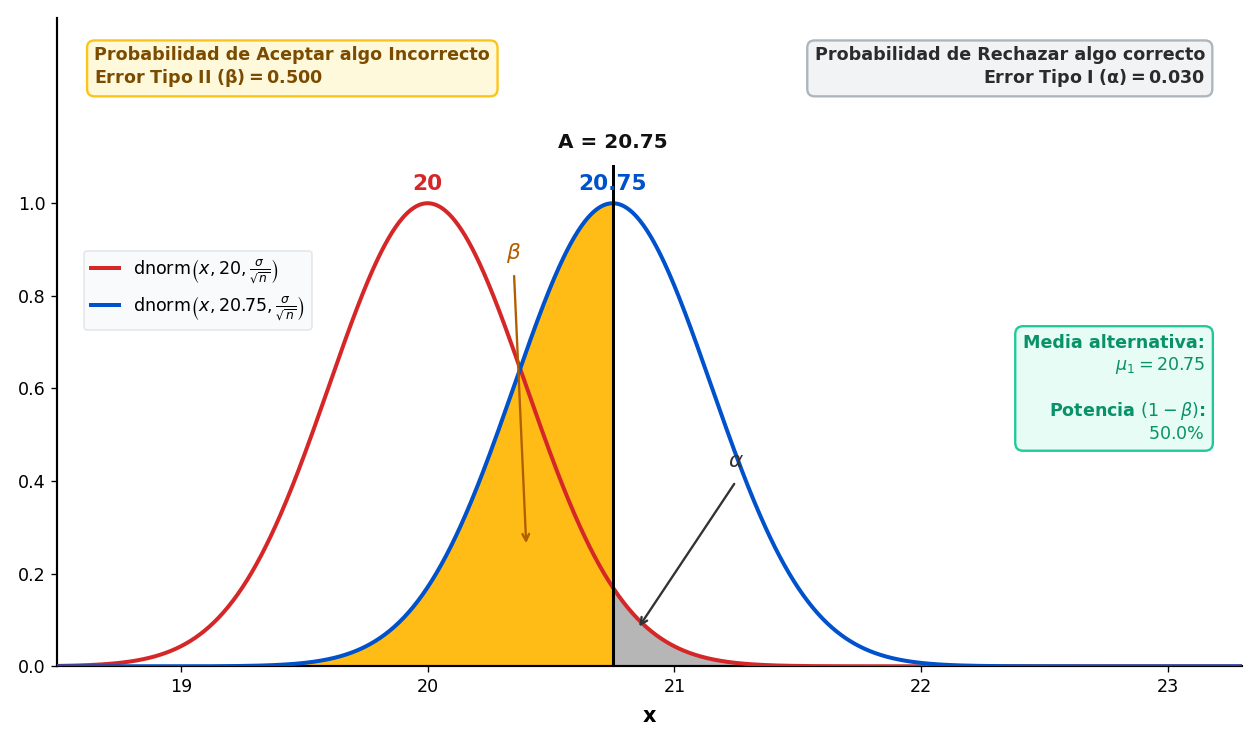
\includegraphics[width=.92\textwidth]{imagenes colas/derecha1.png}
\caption{Cola derecha: región crítica, Error Tipo I y Error Tipo II.}
\end{figure}

Mover la frontera hacia la izquierda aumenta la región de rechazo: disminuye $\beta$, pero aumenta $\alpha$. Moverla hacia la derecha produce el efecto contrario. Con los demás elementos fijos, reducir un error suele aumentar el otro.

\begin{figure}[H]
\centering
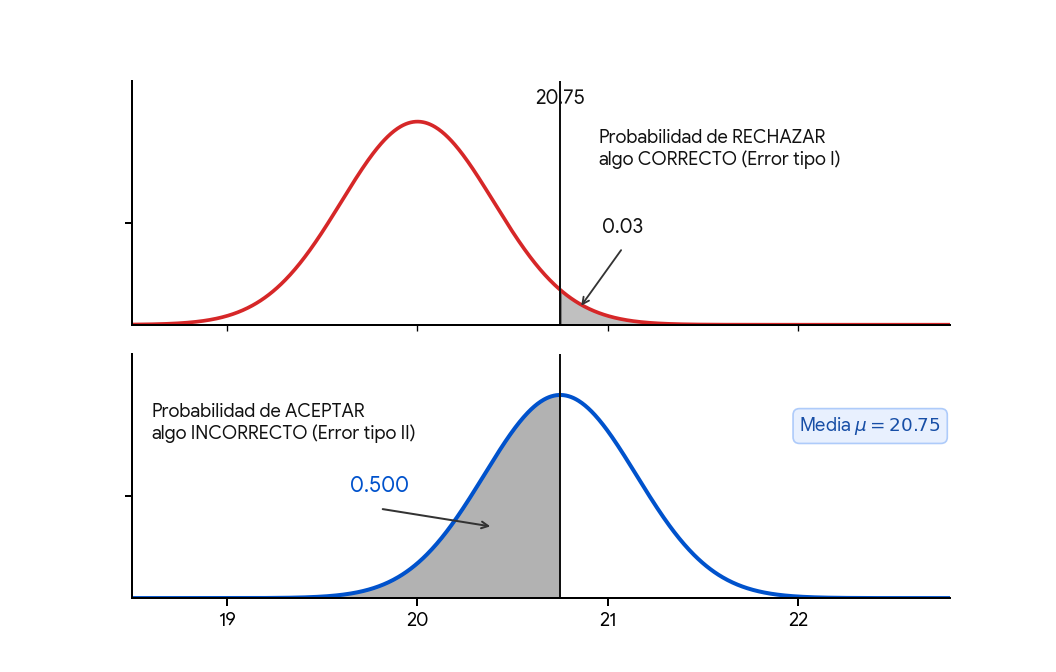
\includegraphics[width=.86\textwidth]{imagenes colas/derecha2.png}
\caption{Descomposición de los errores para una prueba de cola derecha.}
\end{figure}

\subsection{Prueba de cola izquierda}

Con una región de rechazo a la izquierda:
\begin{itemize}
\item cuando $\mu_1$ aumenta y se aleja hacia la derecha de la región crítica, $\beta$ aumenta;
\item cuando $\mu_1$ disminuye y se aleja de $\mu_0$ hacia la izquierda, $\beta$ disminuye y la potencia aumenta.
\end{itemize}

\begin{figure}[H]
\centering
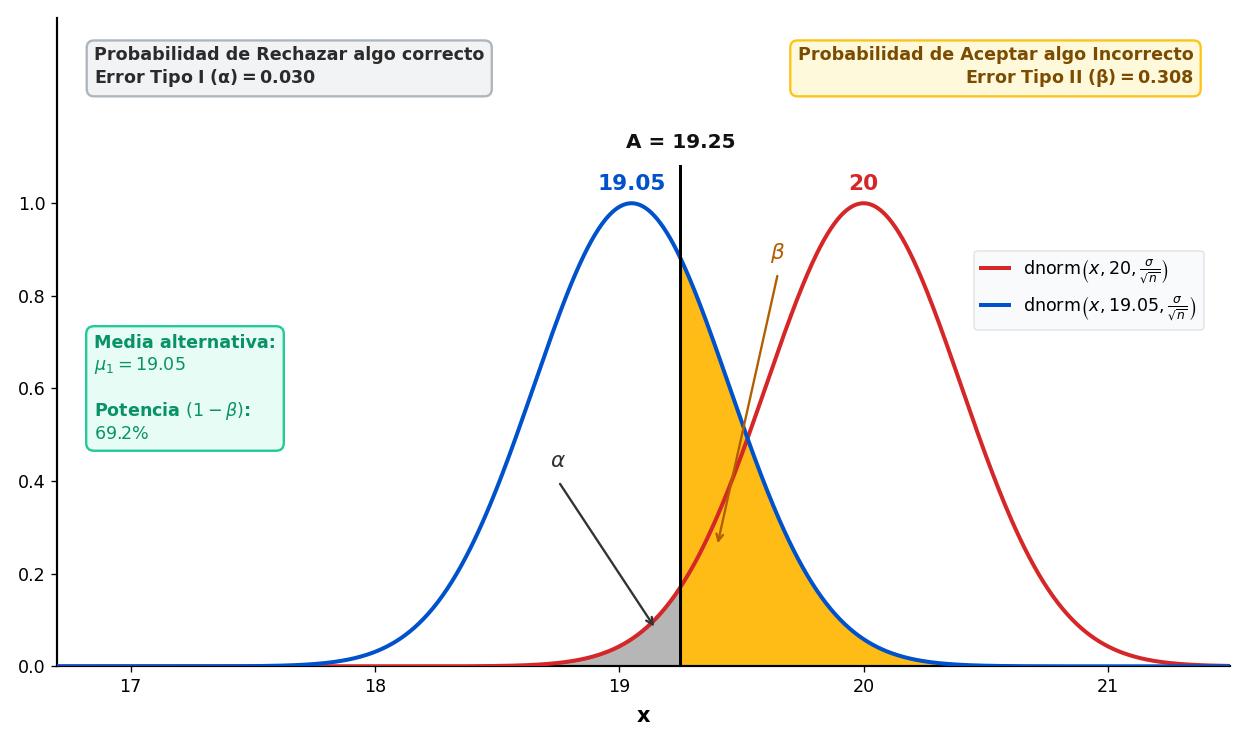
\includegraphics[width=.86\textwidth]{imagenes colas/izquierda1.png}
\caption{Cola izquierda: la región de rechazo se encuentra a la izquierda de la frontera.}
\end{figure}

\begin{figure}[H]
\centering
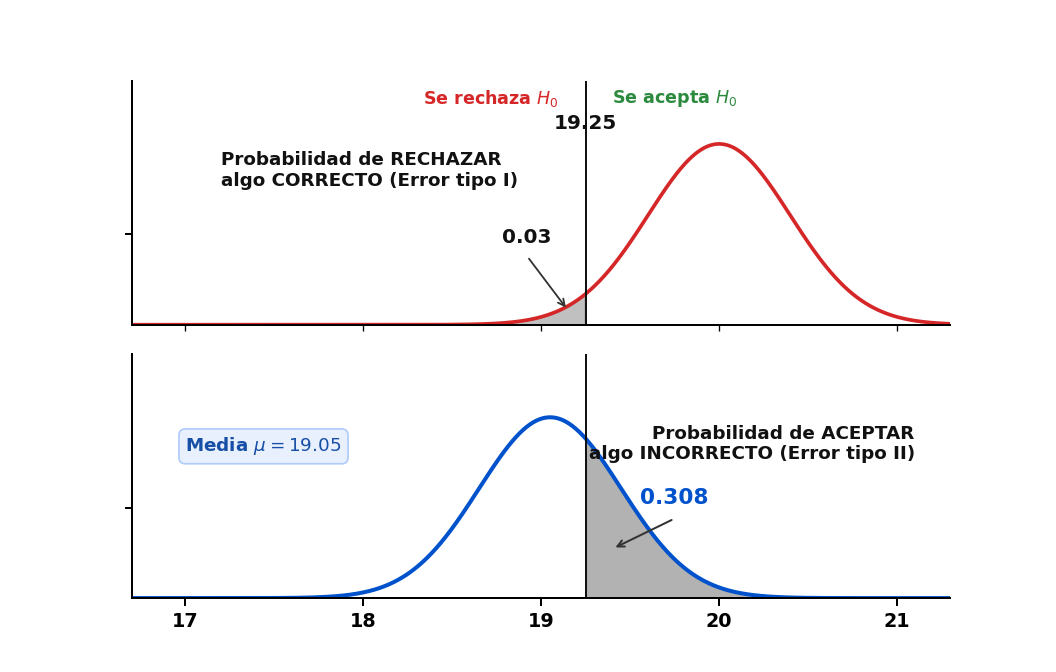
\includegraphics[width=.86\textwidth]{imagenes colas/izquierda2.png}
\caption{Descomposición de los errores para una prueba de cola izquierda.}
\end{figure}

\subsection{Prueba bilateral}

En una prueba bilateral existen dos regiones de rechazo y se coloca $\alpha/2$ en cada cola. La probabilidad de no rechazo es máxima alrededor de $\mu_0$ y disminuye cuando la media real se aleja hacia cualquiera de los dos lados.

Si la media real coincide con $\mu_0$, la probabilidad de no rechazo vale $1-\alpha$. Para alternativas alejadas, $\beta$ disminuye y la potencia se aproxima a $1$.

\begin{figure}[H]
\centering
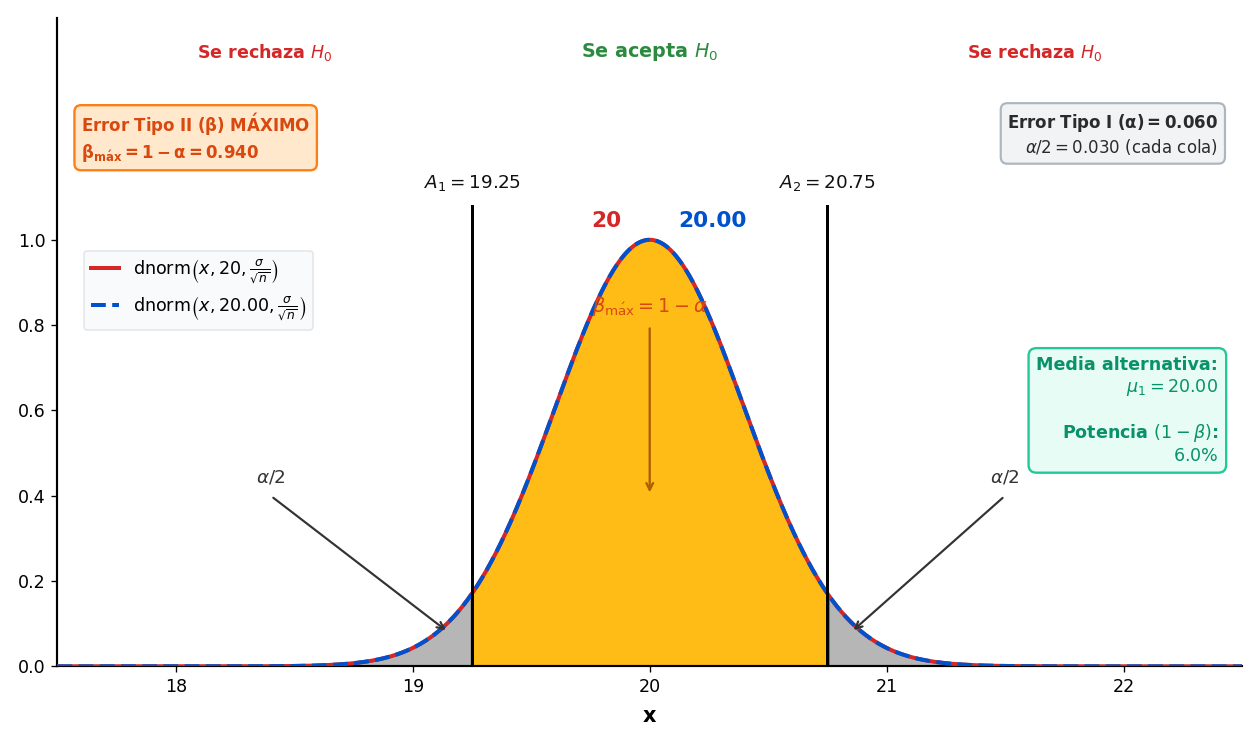
\includegraphics[width=.86\textwidth]{imagenes colas/bilateral1.png}
\caption{Prueba bilateral: $\alpha/2$ en cada cola y región central de no rechazo.}
\end{figure}

\begin{figure}[H]
\centering
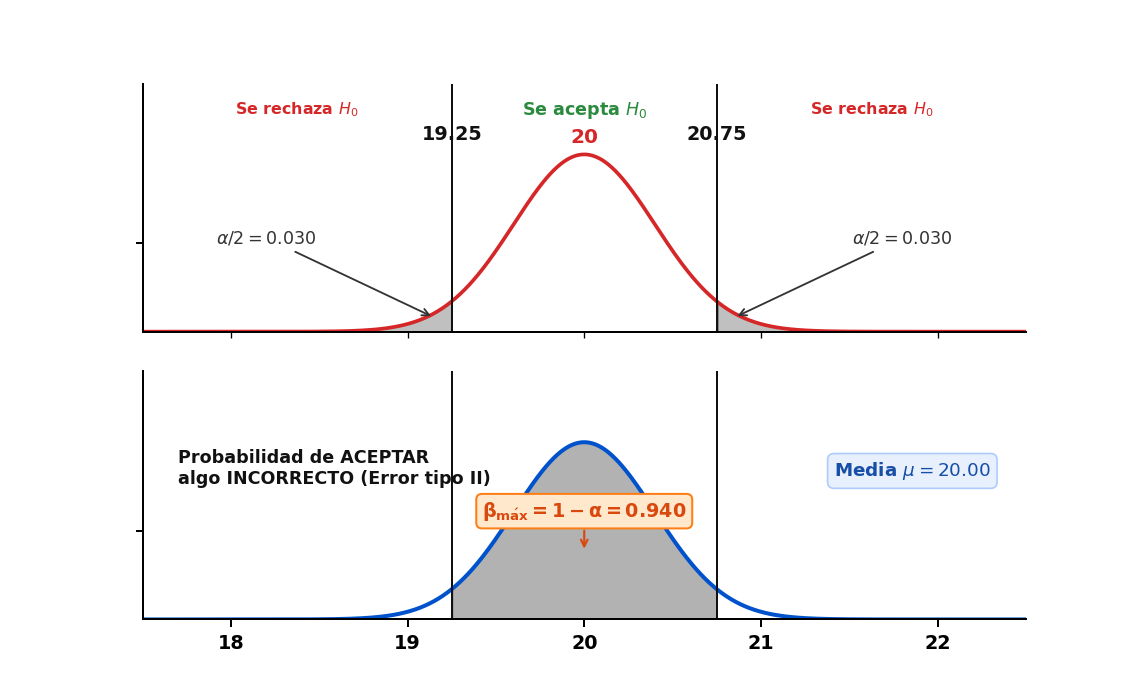
\includegraphics[width=.86\textwidth]{imagenes colas/bilateral2.png}
\caption{Descomposición de los errores para una prueba bilateral.}
\end{figure}

% =============================================================================
\section{Hipótesis relativas a dos medias}

\subsection{Qué problema se quiere resolver}

En esta prueba se comparan las medias de dos poblaciones. El parámetro de interés ya no es una media aislada, sino la \textbf{diferencia entre las medias poblacionales}:
\[
\mu_1-\mu_2.
\]
Por ejemplo, puede interesar saber si un tratamiento produce más que un control, si dos métodos tienen el mismo rendimiento o si una aleación reduce la resistencia en una cantidad determinada.

La hipótesis nula se escribe en forma general como
\[
\Hcero:\mu_1-\mu_2=\delta,
\]
donde $\delta$ es la diferencia propuesta. En la mayoría de las comparaciones se usa $\delta=0$, que representa igualdad de medias; sin embargo, $\delta$ puede ser cualquier diferencia de interés práctico.

\begin{idea}[Cómo comenzar este tema en el examen oral]
``Hasta ahora se estudiaba una media poblacional comparándola con un valor de referencia. En esta parte se comparan dos poblaciones y el parámetro de interés pasa a ser la diferencia $\mu_1-\mu_2$. La lógica de la prueba no cambia: se plantea una hipótesis nula, se elige una alternativa, se fija $\alpha$, se calcula un estadístico y se decide si la diferencia observada es suficientemente grande para rechazar $\Hcero$.''
\end{idea}

Es importante distinguir los parámetros de los estadísticos muestrales:
\[
\underbrace{\mu_1-\mu_2}_{\text{diferencia poblacional que se quiere estudiar}}
\qquad\text{y}\qquad
\underbrace{\bar x_1-\bar x_2}_{\text{diferencia observada en las muestras}}.
\]
La muestra permite decidir si la diferencia observada es compatible con el valor $\delta$ propuesto por $\Hcero$.

\begin{regla}[Antes de elegir una fórmula]
Primero hay que decidir si las observaciones son \textbf{independientes} o \textbf{apareadas}. Si son independientes, se analiza el tamaño de las muestras y si las varianzas poblacionales son conocidas. Para muestras pequeñas, el material de la cátedra desarrolla la prueba $t$ bajo normalidad e igualdad de varianzas.
\end{regla}

\subsection{Muestras independientes y muestras apareadas}

\begin{table}[H]
\centering
\caption{Cómo reconocer la relación entre las muestras.}
\begin{tabularx}{\textwidth}{L{3.1cm}YY}
\toprule
\rowcolor{azulclaro}
\textbf{Tipo} & \textbf{Cómo reconocerlo} & \textbf{Procedimiento}\\
\midrule
Independientes & Las observaciones de un grupo no tienen correspondencia con las del otro. Ejemplo: parcelas tratadas y parcelas de control. & Se analiza directamente $\bar X_1-\bar X_2$ mediante una prueba $Z$ o una prueba $t$ bimuestral.\\
\rowcolor{grisclaro}
Apareadas & Cada dato del primer grupo está vinculado con uno del segundo. Ejemplo: la misma planta industrial antes y después. & Se forman diferencias $d_i$ y se realiza una prueba $t$ para una sola media, $\mu_d$.\\
\bottomrule
\end{tabularx}
\end{table}

\begin{advertencia}[Error frecuente]
No se debe aplicar una prueba para muestras independientes a datos de ``antes y después''. Al ignorar las parejas se pierde la información de cada unidad y se calcula un error estándar que no corresponde al diseño.
\end{advertencia}

\subsection{Elección del estadístico para dos medias}

\begin{table}[H]
\centering
\caption{Cuadro de decisión para dos medias.}
\small
\begin{tabularx}{\textwidth}{L{2.5cm}L{3.2cm}Y L{2.7cm}}
\toprule
\rowcolor{azulclaro}
\textbf{Relación} & \textbf{Información disponible} & \textbf{Condiciones principales} & \textbf{Estadístico}\\
\midrule
Independientes & $\sigma_1$ y $\sigma_2$ conocidas & Poblaciones normales o muestras suficientemente grandes & $Z$ para dos medias\\
\rowcolor{grisclaro}
Independientes & Varianzas desconocidas y muestras grandes & Independencia; aproximación normal por el TCL & $Z$ aproximado usando $s_1,s_2$\\
Independientes & Varianzas desconocidas y muestras pequeñas & Poblaciones normales, $\sigma_1^2=\sigma_2^2$ & $t$ combinada\\
Apareadas & Una diferencia por cada pareja & Diferencias independientes y aproximadamente normales si $n$ es pequeño & $t$ sobre $\bar d$\\
\bottomrule
\end{tabularx}
\end{table}

\clearpage
\begin{landscape}
\pdfpageattr{/Rotate 90}
\thispagestyle{empty}
\subsection{Árbol de decisión para comparar dos medias}

El árbol ocupa una página completa para que puedan leerse las condiciones y las fórmulas. Primero se identifica si los datos están apareados; la rama independiente continúa con el tamaño muestral y las varianzas.

\begin{center}
\resizebox{.86\linewidth}{!}{%
\begin{tikzpicture}[x=1cm,y=1cm]
\node[treelargeq] (par) at (0,0) {¿Las observaciones están apareadas?};

\node[treelargeout] (ap) at (-6.2,-3.8) {\textbf{$t$ apareada}\\[1mm]
Calcular $d_i$ y probar sobre $\mu_d$.\\[1mm]
$\displaystyle t=\frac{\bar d-\mu_{d,0}}{s_d/\sqrt n}$\\[1mm]
$\nu=n-1$.};

\node[treelargeq] (ind) at (6.0,-3.8) {¿$\sigma_1,\sigma_2$ conocidas o ambas muestras grandes?};

\node[treelargeout] (z) at (1.6,-8.1) {\textbf{$Z$ para dos medias}\\[1mm]
$\displaystyle z=\frac{(\bar x_1-\bar x_2)-\delta}
{\sqrt{\sigma_1^2/n_1+\sigma_2^2/n_2}}$\\[1mm]
Con muestras grandes, usar $s_1,s_2$.};

\node[treelargeq] (cond) at (10.7,-8.1) {¿Poblaciones normales y varianzas iguales?};

\node[treelargeout] (tc) at (7.4,-12.5) {\textbf{$t$ bimuestral}\\[1mm]
Usar la varianza combinada $s_p^2$.\\[1mm]
$\displaystyle t=\frac{(\bar x_1-\bar x_2)-\delta}
{s_p\sqrt{1/n_1+1/n_2}}$\\[1mm]
$\nu=n_1+n_2-2$.};

\node[treelargewarn] (rev) at (14.0,-12.5) {\textbf{No aplicar automáticamente}\\[1mm]
No se cumplen las condiciones de la prueba $t$ desarrollada en la guía.\\[1mm]
Revisar los supuestos.};

\draw[arrow] (par)--node[edgeword,above left]{sí}(ap);
\draw[arrow] (par)--node[edgeword,above right]{no}(ind);
\draw[arrow] (ind)--node[edgeword,above left]{sí}(z);
\draw[arrow] (ind)--node[edgeword,above right]{no}(cond);
\draw[arrow] (cond)--node[edgeword,above left]{sí}(tc);
\draw[arrow] (cond)--node[edgeword,above right]{no}(rev);
\end{tikzpicture}%
}
\end{center}

\vfill
\hfill\textcolor{gris}{\thepage}
\end{landscape}
\pdfpageattr{}

\begin{idea}[Idea que unifica todos los casos]
Todo estadístico de esta sección tiene la misma estructura:
\[
\text{estadístico}=
\frac{\text{diferencia observada}-\text{diferencia propuesta en }\Hcero}
{\text{error estándar de la diferencia}}.
\]
Un valor alejado de cero indica que la diferencia observada es grande en relación con la variabilidad esperada por muestreo.
\end{idea}

\subsection{Símbolos que deben explicarse antes de calcular}

\begin{table}[H]
\centering
\caption{Lectura de la notación utilizada al comparar dos medias.}
\small
\begin{tabularx}{\textwidth}{C{2.5cm}Y}
\toprule
\rowcolor{azulclaro}
\textbf{Símbolo} & \textbf{Qué significa y cómo se lee}\\
\midrule
$\mu_1,\mu_2$ & Medias de las dos poblaciones. Son parámetros desconocidos.\\
\rowcolor{grisclaro}
$\bar x_1,\bar x_2$ & Medias calculadas con las muestras 1 y 2.\\
$\sigma_1,\sigma_2$ & Desviaciones estándar poblacionales.\\
\rowcolor{grisclaro}
$s_1,s_2$ & Desviaciones estándar muestrales, usadas para estimar las poblacionales cuando corresponde.\\
$n_1,n_2$ & Cantidades de observaciones de cada muestra.\\
\rowcolor{grisclaro}
$\delta$ & Diferencia entre medias propuesta por $\Hcero$; suele valer cero.\\
$\alpha$ & Nivel de significancia: probabilidad máxima admitida de cometer Error Tipo I.\\
\rowcolor{grisclaro}
$\beta$ & Probabilidad de no rechazar $\Hcero$ cuando una diferencia alternativa es verdadera.\\
$\nu$ & Grados de libertad de la distribución $t$.\\
\bottomrule
\end{tabularx}
\end{table}

\begin{regla}[Frase de transición para el oral]
``Una vez definido que el parámetro es $\mu_1-\mu_2$, debo identificar si las muestras son independientes o apareadas, porque esa decisión determina la forma del error estándar y, por lo tanto, el estadístico que corresponde.''
\end{regla}

\subsection{Dos muestras independientes: distribución de la diferencia}

Sean dos muestras aleatorias independientes de tamaños $n_1$ y $n_2$. Se define
\[
D=\bar X_1-\bar X_2.
\]
Como las muestras son independientes,
\[
E(D)=\mu_1-\mu_2,
\qquad
\operatorname{Var}(D)=\frac{\sigma_1^2}{n_1}+\frac{\sigma_2^2}{n_2},
\]
y, por lo tanto,
\[
\EE(D)=\sqrt{\frac{\sigma_1^2}{n_1}+\frac{\sigma_2^2}{n_2}}.
\]
La diferencia es normal si ambas poblaciones son normales. Con muestras grandes puede utilizarse la aproximación normal por el teorema central del límite.

Cuando las desviaciones poblacionales son conocidas, para contrastar $\Hcero:\mu_1-\mu_2=\delta$ se usa
\[
z=\frac{(\bar x_1-\bar x_2)-\delta}
{\sqrt{\dfrac{\sigma_1^2}{n_1}+\dfrac{\sigma_2^2}{n_2}}}.
\]
Si las muestras son grandes y las varianzas poblacionales son desconocidas, el criterio del apunte reemplaza $\sigma_1$ y $\sigma_2$ por $s_1$ y $s_2$:
\[
z\approx\frac{(\bar x_1-\bar x_2)-\delta}
{\sqrt{\dfrac{s_1^2}{n_1}+\dfrac{s_2^2}{n_2}}}.
\]

\begin{idea}[Cómo leer la fórmula]
\begin{itemize}
\item $\bar x_1,\bar x_2$: medias observadas; $\mu_1,\mu_2$: medias poblacionales.
\item $n_1,n_2$: tamaños de las muestras independientes.
\item $\sigma_1^2,\sigma_2^2$: varianzas poblacionales; $s_1^2,s_2^2$: estimaciones muestrales.
\item $\delta$: diferencia que se supone cierta en $\Hcero$; suele ser cero.
\item El denominador es el error estándar de $\bar X_1-\bar X_2$ y $z$ expresa cuántos errores estándar separan la diferencia observada de $\delta$.
\end{itemize}
En palabras, se lee: ``diferencia observada entre las medias muestrales, menos la diferencia planteada por la hipótesis nula, dividido por el error estándar de la diferencia''.
\end{idea}

\begin{regla}[Qué justificar oralmente]
Las varianzas se \textbf{suman} aunque las medias se resten. Esto ocurre porque la variabilidad de las dos medias muestrales aporta incertidumbre a la diferencia. Para muestras independientes, la varianza de la diferencia es la suma de ambas varianzas.
\end{regla}

\subsection{Formulación de hipótesis y regiones críticas}

El orden de los grupos importa. Si se define la diferencia como $\mu_1-\mu_2$, todas las hipótesis y todos los cálculos deben mantener ese mismo orden.

\begin{table}[H]
\centering
\caption{Regiones de rechazo para dos medias.}
\begin{tabularx}{.92\textwidth}{YY}
\toprule
\rowcolor{azulclaro}
\textbf{Hipótesis alternativa} & \textbf{Rechazar $\Hcero$ si}\\
\midrule
$\Huno:\mu_1-\mu_2<\delta$ & $z_{calc}<-z_\alpha$\\
\rowcolor{grisclaro}
$\Huno:\mu_1-\mu_2>\delta$ & $z_{calc}>z_\alpha$\\
$\Huno:\mu_1-\mu_2\ne\delta$ & $|z_{calc}|>z_{\alpha/2}$\\
\bottomrule
\end{tabularx}
\end{table}

Para una prueba $t$ se conserva la misma lógica, pero se reemplazan los valores críticos normales por los valores de la distribución $t$ con los grados de libertad correspondientes.

\subsection{Comandos esenciales para los valores críticos en R}

R puede reemplazar la búsqueda en tablas una vez elegidas la distribución y la cola:
\[
\begin{array}{lll}
Z\text{ derecha:} & \texttt{qnorm(1-alpha)}, &
Z\text{ bilateral:} \ \texttt{qnorm(1-alpha/2)},\\[1mm]
t\text{ derecha:} & \texttt{qt(1-alpha, df=nu)}, &
t\text{ bilateral:} \ \texttt{qt(1-alpha/2, df=nu)}.
\end{array}
\]
Para cola izquierda se usa \texttt{qnorm(alpha)} o \texttt{qt(alpha, df=nu)}. R realiza el cálculo numérico, pero la elección de la prueba y de los grados de libertad debe justificarse previamente. El desarrollo completo y los ejemplos reproducibles se encuentran en el anexo ``Resolución con R''.

\subsection{Ejemplo I: resistencia de conductores}

Se desea verificar si una aleación reduce la resistencia en más de $0.050$ ohms. Se toma como población 1 el alambre ordinario y como población 2 el alambre con aleación:
\[
n_1=n_2=32,\quad \bar x_1=0.136,\quad s_1=0.004,
\qquad \bar x_2=0.083,\quad s_2=0.005.
\]
Como ambas muestras son grandes, se usa la aproximación normal con $s_1$ y $s_2$.

\begin{enumerate}[label=\textbf{\arabic*.}]
\item \textbf{Hipótesis:}
\[
\Hcero:\mu_1-\mu_2=0.050,
\qquad
\Huno:\mu_1-\mu_2>0.050.
\]
\item \textbf{Nivel y región crítica:} $\alpha=0.05$, cola derecha; rechazar si $z>1.645$.
\item \textbf{Cálculo:}
\[
z=\frac{(0.136-0.083)-0.050}
{\sqrt{0.004^2/32+0.005^2/32}}
\approx2.65.
\]
\item \textbf{Decisión:} como $2.65>1.645$, se rechaza $\Hcero$.
\end{enumerate}

\begin{conclusion}
Con un nivel de significancia de $0.05$, existe evidencia suficiente para sostener que la aleación reduce la resistencia del conductor en más de $0.050$ ohms.
\end{conclusion}

\textbf{R, cálculo esencial:} calcular \texttt{z\_calc} con la fórmula anterior y obtener el crítico mediante \texttt{qnorm(0.95)}. Se obtiene $2.65>1.645$. El código completo está en el anexo.

\begin{idea}[Cómo presentarlo oralmente]
``Son dos muestras independientes y grandes; por eso uso $Z$ y reemplazo las desviaciones poblacionales por las muestrales, como indica la guía. La alternativa tiene signo mayor, de modo que la prueba es de cola derecha. Como $z_{calc}=2.65$ supera a $z_{crit}=1.645$, rechazo $\Hcero$ y concluyo que la reducción supera significativamente $0.050$ ohms.''
\end{idea}

\subsection{Ejemplo II: estatura de estudiantes}

Se comparan $50$ estudiantes que participan en pruebas atléticas (grupo 1) con $50$ que no participan (grupo 2):
\[
\bar x_1=1.70,\quad s_1=0.0625,
\qquad
\bar x_2=1.687,\quad s_2=0.07.
\]
Se quiere determinar si la media del primer grupo es mayor.

\begin{enumerate}[label=\textbf{\arabic*.}]
\item $\Hcero:\mu_1-\mu_2=0$; $\Huno:\mu_1-\mu_2>0$.
\item $\alpha=0.05$; cola derecha; rechazar si $z>1.645$.
\item
\[
z=\frac{1.70-1.687}
{\sqrt{0.0625^2/50+0.07^2/50}}
\approx0.98.
\]
\item Como $0.98<1.645$, no se rechaza $\Hcero$.
\end{enumerate}

\begin{conclusion}
La muestra no aporta evidencia suficiente para concluir que los estudiantes que participan en pruebas atléticas sean, en promedio, más altos que los demás. No rechazar $\Hcero$ no demuestra que las medias sean iguales.
\end{conclusion}

\begin{idea}[Posible repregunta]
\textbf{¿Por qué no se acepta $\Hcero$?} Porque el resultado solo indica que la evidencia muestral no fue suficiente para rechazarla con $\alpha=0.05$. No demuestra que las medias poblacionales sean exactamente iguales.
\end{idea}

\subsection{Error Tipo II y potencia para dos medias}

El Error Tipo II se estudia fijando una diferencia real alternativa $\delta'=\mu_1-\mu_2$. Para conectar el problema con las curvas características de operación, el apunte usa
\[
d=\frac{|\delta-\delta'|}{\sqrt{\sigma_1^2+\sigma_2^2}}.
\]
Cuanto más lejos esté $\delta'$ de la diferencia nula $\delta$, más sencillo será detectar el cambio: $\beta$ disminuye y la potencia $1-\beta$ aumenta.

En el ejemplo de estaturas, para $\delta'=0.02$ m:
\[
d=\frac{|0-0.02|}{\sqrt{0.0625^2+0.07^2}}
\approx0.213.
\]
Con $\alpha=0.05$ y $n_1=n_2=50$, el material obtiene
\[
\beta\approx0.5549,
\qquad
1-\beta\approx0.4451.
\]
Esto significa que, si la diferencia real fuera $0.02$ m, la prueba tendría aproximadamente un $44.51\%$ de probabilidad de detectarla con la regla de decisión establecida.

Si $n_1\ne n_2$, el tamaño equivalente indicado por el apunte es
\[
n_{eq}=\frac{\sigma_1^2+\sigma_2^2}
{\dfrac{\sigma_1^2}{n_1}+\dfrac{\sigma_2^2}{n_2}}.
\]

\begin{idea}[Cómo explicarlo sin perderse en la fórmula]
``El Error Tipo II consiste en no detectar una diferencia que realmente existe. Para una diferencia alternativa $\delta'$, la curva característica de operación permite obtener $\beta$. En este ejemplo, $\beta=0.5549$: si la diferencia real fuera $0.02$ m, habría un $55.49\%$ de probabilidad de no detectarla y una potencia de $44.51\%$. Cuando la diferencia real se aleja de la planteada en $\Hcero$, $\beta$ disminuye y la potencia aumenta.''
\end{idea}

\subsection{Muestras pequeñas independientes: prueba \texorpdfstring{$t$}{t} combinada}

Cuando una o ambas muestras son pequeñas, las varianzas poblacionales son desconocidas y se supone que las dos poblaciones son normales con varianzas iguales, $\sigma_1^2=\sigma_2^2$, se estima la varianza común mediante
\[
s_p^2=
\frac{(n_1-1)s_1^2+(n_2-1)s_2^2}{n_1+n_2-2}.
\]
Esta es una media ponderada de las dos varianzas muestrales: cada una recibe un peso proporcional a sus grados de libertad. El error estándar estimado es
\[
\EE(\bar X_1-\bar X_2)
=s_p\sqrt{\frac1{n_1}+\frac1{n_2}}.
\]
El estadístico de prueba resulta
\[
t=\frac{(\bar x_1-\bar x_2)-\delta}
{s_p\sqrt{\dfrac1{n_1}+\dfrac1{n_2}}},
\qquad
\nu=n_1+n_2-2.
\]

\begin{idea}[Significado de los símbolos nuevos]
$s_p^2$ es la varianza muestral combinada, $s_p$ es la desviación estándar combinada y $\nu$ representa los grados de libertad de la distribución $t$. La combinación solo tiene sentido si es razonable suponer una varianza poblacional común.
\end{idea}

\begin{regla}[Cómo leer la prueba $t$ bimuestral]
Se lee: ``diferencia entre las medias muestrales, menos la diferencia propuesta en $\Hcero$, dividido por el error estándar estimado con la desviación combinada''. Los grados de libertad se suman como $(n_1-1)+(n_2-1)=n_1+n_2-2$.
\end{regla}

\subsection{Ejemplo III: fertilizante y producción de trigo}

Se comparan $12$ parcelas tratadas con fertilizante (grupo 1) y $12$ parcelas de control (grupo 2):
\[
n_1=n_2=12,\quad
\bar x_1=0.280,\quad s_1=0.022,
\qquad
\bar x_2=0.264,\quad s_2=0.020.
\]
Se supone normalidad y varianzas poblacionales iguales. Se quiere probar si el fertilizante aumenta la producción.

\begin{enumerate}[label=\textbf{\arabic*.}]
\item $\Hcero:\mu_1-\mu_2=0$; $\Huno:\mu_1-\mu_2>0$.
\item $\alpha=0.05$, cola derecha y $\nu=12+12-2=22$; $t_{crit}=1.717$.
\item Varianza y desviación estándar combinadas:
\[
s_p^2=
\frac{11(0.022)^2+11(0.020)^2}{22}
\approx0.000442,
\qquad
s_p\approx0.02102.
\]
\item Estadístico:
\[
t=\frac{0.280-0.264}
{0.02102\sqrt{1/12+1/12}}
\approx1.864.
\]
\item Como $1.864>1.717$, se rechaza $\Hcero$.
\end{enumerate}

\begin{advertencia}[Diferencia numérica con el apunte]
El material original informa $t_{calc}=1.849$. Al calcular con los datos impresos, $s_p^2=0.000442$ y $s_p\approx0.02102$, se obtiene $t_{calc}\approx1.864$. Los dos valores superan $1.717$, por lo que la decisión y la conclusión no cambian.
\end{advertencia}

\begin{conclusion}
Al nivel de significancia del $5\%$, existe evidencia suficiente para concluir que el fertilizante incrementa la producción media de trigo.
\end{conclusion}

\textbf{R, cálculo esencial:} obtener primero \texttt{sp2}, calcular \texttt{t\_calc} con la fórmula anterior y usar \texttt{qt(0.95, df=22)} para el crítico. R devuelve $1.864>1.717$. El código completo está en el anexo.

\begin{idea}[Cómo presentarlo oralmente]
``Las dos muestras son independientes y pequeñas. Como se supone normalidad e igualdad de varianzas poblacionales, corresponde una $t$ bimuestral. Primero estimo la varianza común con $s_p^2$ y después calculo el estadístico con $\nu=12+12-2=22$. Como $1.864$ supera el crítico $1.717$, rechazo $\Hcero$ y concluyo que el fertilizante incrementa significativamente la producción.''
\end{idea}

\subsection{Muestras apareadas: prueba sobre la media de las diferencias}

En datos apareados las dos mediciones no son independientes: cada observación del primer conjunto está vinculada con una del segundo. Por eso no se comparan como si fueran dos grupos separados. Se calcula, para cada unidad,
\[
d_i=x_{\text{antes},i}-x_{\text{después},i}.
\]
Después se trabaja como en una prueba de una sola media:
\[
\bar d=\frac{\sum_{i=1}^{n}d_i}{n},
\qquad
s_d=\sqrt{\frac{\sum_{i=1}^{n}(d_i-\bar d)^2}{n-1}},
\]
\[
t=\frac{\bar d-\mu_{d,0}}{s_d/\sqrt n},
\qquad
\nu=n-1.
\]

\begin{idea}[Cómo interpretar las diferencias]
$d_i$ es la diferencia dentro de la pareja $i$; $\bar d$ estima la diferencia media poblacional $\mu_d$; $s_d$ mide cuánto varían las diferencias. El signo elegido para $d_i$ determina la dirección de $\Huno$. Si se define $d_i=\text{antes}-\text{después}$, una reducción produce valores positivos.
\end{idea}

\begin{regla}[Cómo leer la fórmula]
Se lee: ``media observada de las diferencias, menos la diferencia media propuesta por $\Hcero$, dividido por el error estándar de las diferencias''. El tamaño muestral $n$ es la cantidad de \textbf{parejas}, y los grados de libertad son $n-1$.
\end{regla}

\begin{advertencia}[Distinción que suelen preguntar]
En la $t$ bimuestral se comparan dos medias de muestras independientes. En la $t$ apareada se construye una sola muestra formada por los $d_i$ y se contrasta la media poblacional de esas diferencias. Por eso sus errores estándar y sus grados de libertad no son iguales.
\end{advertencia}

\subsection{Ejemplo IV: programa de seguridad}

Se registran las horas-hombre perdidas por accidentes en las mismas $10$ plantas antes y después de aplicar un programa. Se define $d_i=\text{antes}-\text{después}$:

\begin{table}[H]
\centering
\caption{Horas-hombre perdidas antes y después del programa.}
\begingroup
\scriptsize
\setlength{\tabcolsep}{4pt}
\begin{tabular}{c*{10}{c}}
\toprule
\rowcolor{azulclaro}
\textbf{Planta} & 1 & 2 & 3 & 4 & 5 & 6 & 7 & 8 & 9 & 10\\
\midrule
Antes   & 45 & 73 & 46 & 124 & 33 & 57 & 83 & 34 & 26 & 17\\
Después & 36 & 60 & 44 & 119 & 35 & 51 & 77 & 29 & 24 & 11\\
\rowcolor{grisclaro}
$d_i$   & 9  & 13 & 2  & 5   & $-2$ & 6 & 6 & 5 & 2 & 6\\
\bottomrule
\end{tabular}
\endgroup
\end{table}

Si el programa es eficaz, las pérdidas posteriores serán menores y la diferencia media será positiva.

\begin{enumerate}[label=\textbf{\arabic*.}]
\item \textbf{Hipótesis:} $\Hcero:\mu_d=0$; $\Huno:\mu_d>0$.

\item \textbf{Nivel, cola y valor crítico:} $\alpha=0.05$, cola derecha y $\nu=10-1=9$; por lo tanto, $t_{crit}=1.833$.

\item \textbf{Fórmula para trabajar con la tabla normalizada:}
\[
t=\frac{\bar d-\mu_{d,0}}{s_d/\sqrt n}.
\]
En este caso, $\bar d$ es la media de la muestra de diferencias, $s_d$ es su desviación estándar, $\mu_{d,0}=0$ y $n=10$ es la cantidad de parejas.

\item \textbf{Media y desviación estándar de la muestra de diferencias:}
\[
\bar d=
\frac{9+13+2+5-2+6+6+5+2+6}{10}
=\frac{52}{10}=5.2.
\]
Para la desviación estándar se utiliza la forma de cálculo equivalente
\[
s_d=\sqrt{\frac{\sum d_i^2-n\bar d^{,2}}{n-1}}.
\]
Primero,
\[
\sum d_i^2
=9^2+13^2+2^2+5^2+(-2)^2+6^2+6^2+5^2+2^2+6^2
=420.
\]
Luego,
\[
s_d=\sqrt{\frac{420-10(5.2)^2}{9}}
=\sqrt{16.6222}\approx4.077.
\]

\item \textbf{Estadístico calculado:}
\[
t=\frac{5.2-0}{4.077/\sqrt{10}}
\approx4.033.
\]

\item \textbf{Decisión:} como $4.033>1.833$, se rechaza $\Hcero$.
\end{enumerate}

\begin{conclusion}
Con un nivel de significancia de $0.05$, existe evidencia suficiente para concluir que el programa de seguridad reduce las horas-hombre perdidas por accidentes.
\end{conclusion}

\textbf{R, cálculo esencial:} \texttt{d <- antes-despues}, \texttt{t\_calc <- mean(d)/(sd(d)/sqrt(length(d)))} y \texttt{t\_crit <- qt(0.95, df=9)}. R devuelve $4.033>1.833$. El bloque completo está en el anexo.

\begin{idea}[Cómo presentarlo oralmente]
``Las mediciones están apareadas porque corresponden a las mismas diez plantas antes y después. Defino $d_i=\text{antes}-\text{después}$; por lo tanto, si el programa reduce las pérdidas, espero diferencias positivas y planteo $\Huno:\mu_d>0$. Trabajo con una sola muestra de diez diferencias, de modo que uso una $t$ con nueve grados de libertad. Como $4.033>1.833$, rechazo $\Hcero$ y concluyo que el programa es eficaz.''
\end{idea}

\subsection{Errores frecuentes y guía para el examen}

\begin{itemize}
\item \textbf{Cambiar el orden de los grupos:} si se define $\mu_1-\mu_2$, mantener ese orden en hipótesis, datos y conclusión.
\item \textbf{Confundir independencia con apareamiento:} en antes/después se analizan diferencias, no dos medias independientes.
\item \textbf{Usar la $t$ combinada sin mencionar sus condiciones:} para muestras pequeñas, la guía exige independencia, normalidad e igualdad de varianzas poblacionales.
\item \textbf{Olvidar $\delta$:} el numerador siempre resta la diferencia propuesta por $\Hcero$, aunque sea distinta de cero.
\item \textbf{Decir que se ``acepta'' $\Hcero$:} la expresión correcta es ``no se rechaza'', porque la falta de evidencia no demuestra igualdad.
\item \textbf{Dar una conclusión puramente numérica:} finalizar siempre hablando de las dos poblaciones estudiadas.
\item \textbf{Restar las varianzas porque se restan las medias:} para muestras independientes, las varianzas del error se suman.
\item \textbf{Usar $n_1+n_2-2$ en datos apareados:} la prueba apareada tiene $n-1$ grados de libertad porque se analiza una sola muestra de $n$ diferencias.
\end{itemize}

\begin{regla}[Secuencia para explicar el tema oralmente]
\begin{enumerate}[label=\textbf{\arabic*.}]
\item Identificar las dos poblaciones y definir el orden de la diferencia.
\item Decidir si las muestras son independientes o apareadas.
\item Escribir $\Hcero$ y $\Huno$; el signo de $\Huno$ determina la cola.
\item Verificar normalidad, tamaños muestrales y tratamiento de las varianzas.
\item Elegir $Z$, $t$ bimuestral combinada o $t$ apareada y explicar por qué.
\item Calcular el error estándar y el estadístico.
\item Comparar el estadístico calculado con el valor crítico correspondiente.
\item Redactar la conclusión en el contexto y recordar que no rechazar no prueba igualdad.
\end{enumerate}
\end{regla}

\subsection{Preguntas breves que pueden aparecer en el oral}

\begin{description}[style=nextline,itemsep=7pt]
\item[¿Qué cambia respecto de una prueba sobre una media?]
El parámetro pasa de ser $\mu$ a ser $\mu_1-\mu_2$, y el error estándar debe incorporar la variabilidad de las dos medias muestrales.

\item[¿Por qué importa el orden de los grupos?]
Porque cambiar $\mu_1-\mu_2$ por $\mu_2-\mu_1$ cambia el signo de la diferencia y, por lo tanto, la forma de expresar la alternativa.

\item[¿Por qué se suman las varianzas si las medias se restan?]
Porque ambas muestras aportan incertidumbre. Bajo independencia, la varianza de una suma o de una diferencia es la suma de las varianzas.

\item[¿Cuándo se usa $Z$?]
Cuando las desviaciones poblacionales son conocidas o, según el criterio de la guía, cuando ambas muestras son grandes y se reemplazan por $s_1$ y $s_2$.

\item[¿Cuándo se usa la $t$ bimuestral?]
Cuando las muestras independientes son pequeñas, las poblaciones son normales, las varianzas poblacionales son desconocidas y se suponen iguales.

\item[¿Qué significa $s_p^2$?]
Es la estimación combinada de la varianza poblacional común, ponderada por los grados de libertad de las dos muestras.

\item[¿Por qué una prueba apareada se transforma en unimuestral?]
Porque cada pareja produce una diferencia $d_i$ y el análisis se realiza sobre la única muestra formada por esas diferencias.

\item[¿Qué significa no rechazar $\Hcero$?]
Que la muestra no aporta evidencia suficiente para rechazarla con el nivel de significancia fijado; no significa que se haya demostrado su verdad.
\end{description}

% =============================================================================
\section{Resumen general}

Esta secuencia permite exponer la unidad completa sin enumerar fórmulas aisladas. Cada bloque conduce al siguiente.

\begin{enumerate}[label=\textbf{\arabic*.},leftmargin=2em]
\item \textbf{Comenzar por la idea de prueba de hipótesis.} Explicar que se formula una hipótesis nula sobre un parámetro poblacional y se usa una muestra para decidir si existe evidencia suficiente para rechazarla.

\item \textbf{Definir $\Hcero$ y $\Huno$.} $\Hcero$ contiene la igualdad y representa el punto de partida. $\Huno$ expresa lo que se busca detectar y su signo determina si la prueba es de cola derecha, izquierda o bilateral.

\item \textbf{Presentar el nivel de significancia.} $\alpha$ es la probabilidad de cometer Error Tipo I: rechazar $\Hcero$ cuando es verdadera. Debe fijarse antes de observar la decisión final.

\item \textbf{Explicar el procedimiento general.} Definir el parámetro, formular las hipótesis, elegir $\alpha$, seleccionar el estadístico, determinar la región crítica, calcular y concluir en el contexto.

\item \textbf{Elegir la distribución para una media.} Justificar el uso de $Z$ o $t$ según el tamaño muestral, la normalidad y el conocimiento de la varianza poblacional. Mostrar que el estadístico compara la distancia entre $\bar x$ y $\mu_0$ con su error estándar.

\item \textbf{Relacionar región crítica y decisión.} El signo de $\Huno$ ubica la región de rechazo. Si el estadístico calculado entra en ella se rechaza $\Hcero$; de lo contrario, no se rechaza.

\item \textbf{Distinguir los dos errores.} El Error Tipo I tiene probabilidad $\alpha$; el Error Tipo II tiene probabilidad $\beta$. La potencia $1-\beta$ mide la capacidad de detectar una alternativa verdadera.

\item \textbf{Explicar las curvas características de operación.} La curva muestra la probabilidad de no rechazar $\Hcero$ para distintos valores reales del parámetro. Al alejarse la alternativa de la hipótesis nula, suele disminuir $\beta$ y aumentar la potencia. Un tamaño muestral mayor también mejora la capacidad de detección.

\item \textbf{Pasar de una media a dos medias.} El nuevo parámetro es $\mu_1-\mu_2$. La estructura lógica se conserva, pero cambia el error estándar porque ahora intervienen dos muestras.

\item \textbf{Separar muestras independientes y apareadas.} Para muestras independientes se estudia directamente $\bar X_1-\bar X_2$. Para datos vinculados se forman diferencias $d_i$ y se realiza una prueba sobre $\mu_d$.

\item \textbf{Elegir el estadístico para dos medias independientes.} Usar $Z$ con varianzas conocidas o muestras grandes. Para muestras pequeñas, normales y con varianzas iguales desconocidas, usar la $t$ bimuestral y la varianza combinada $s_p^2$.

\item \textbf{Cerrar con la interpretación.} Comparar el estadístico calculado con el crítico y expresar la decisión en palabras del problema. No rechazar $\Hcero$ nunca equivale a demostrar que sea verdadera.
\end{enumerate}

\begin{regla}[Versión breve para memorizar el recorrido]
Concepto de hipótesis $\longrightarrow$ $\Hcero$ y $\Huno$ $\longrightarrow$ colas y $\alpha$ $\longrightarrow$ elección de $Z$ o $t$ $\longrightarrow$ región crítica y decisión $\longrightarrow$ errores $\alpha$ y $\beta$ $\longrightarrow$ curvas C.O. $\longrightarrow$ comparación de dos medias $\longrightarrow$ independientes o apareadas $\longrightarrow$ conclusión en el contexto.
\end{regla}

\subsection{Cuadro final de elección para dos medias}

\begin{table}[H]
\centering
\caption{Resumen para seleccionar el procedimiento al comparar dos medias.}
\small
\begin{tabularx}{\textwidth}{L{3.0cm}Y L{3.4cm}L{2.1cm}}
\toprule
\rowcolor{azulclaro}
\textbf{Datos} & \textbf{Condiciones de la guía} & \textbf{Qué se analiza} & \textbf{Estadístico}\\
\midrule
Independientes & $\sigma_1,\sigma_2$ conocidas o muestras grandes & $\bar X_1-\bar X_2$ & $Z$\\
\rowcolor{grisclaro}
Independientes & Muestras pequeñas, poblaciones normales y varianzas iguales desconocidas & $\bar X_1-\bar X_2$ usando $s_p^2$ & $t$, $\nu=n_1+n_2-2$\\
Apareados & Una medición vinculada con otra dentro de cada pareja & Diferencias $d_i$ y su media $\bar d$ & $t$, $\nu=n-1$\\
\bottomrule
\end{tabularx}
\end{table}

\begin{idea}[Modelo de cierre oral]
``En síntesis, una prueba de hipótesis compara lo observado con lo que debería ocurrir si $\Hcero$ fuera cierta. La diferencia se expresa en unidades de error estándar y se compara con una región crítica fijada mediante $\alpha$. En dos medias, la decisión principal es reconocer si las muestras son independientes o apareadas y, luego, elegir $Z$ o $t$ según la información disponible y los supuestos. Finalmente, la conclusión debe referirse al problema y no limitarse al resultado numérico.''
\end{idea}

\begin{regla}
No rechazar $\Hcero$ no equivale a demostrar que sea verdadera. Solo indica que la muestra no aporta evidencia suficiente para rechazarla con el nivel de significancia elegido.
\end{regla}

% =============================================================================
\clearpage
\section{Anexo: Resolución con R}

\begingroup
\small
\setlength{\parskip}{2pt}
Estas funciones sirven para obtener valores críticos, límites en unidades reales o alturas de una curva. El estadístico calculado $z_{calc}$ o $t_{calc}$ se obtiene con la fórmula de la prueba y luego se compara con el valor crítico devuelto por R.

\rsubentry{Cuantil de la distribución normal: qnorm()}
\begin{rcheat}{\thesubsection\quad Cálculo en R con \texttt{qnorm()}}
\textbf{Qué recibe y qué devuelve.} La instrucción
\texttt{qnorm(p, mean, sd)} recibe tres parámetros y devuelve la abscisa $x_p$ que deja a su izquierda un área acumulada $p$:
\[
x_p=\operatorname{qnorm}(p,\mu,\sigma)
\quad\Longleftrightarrow\quad
P(X\leq x_p)=p.
\]
\begin{rscript}
qnorm(0.05, mean = 0, sd = 1)   \# cola izquierda\par
qnorm(0.95, mean = 0, sd = 1)   \# cola derecha
\end{rscript}
\begin{rverdict}
\textbf{Resultado:}
$\operatorname{qnorm}(0.05,0,1)=-1.644854\approx-1.645$ y
$\operatorname{qnorm}(0.95,0,1)=1.644854\approx1.645$.
Por ejemplo, $P(Z\leq-1.645)=0.05$.
\end{rverdict}
\textbf{Lectura de los parámetros:}
$p$ es el área acumulada desde $-\infty$; \texttt{mean} es la media; y \texttt{sd} es la desviación estándar.
Para obtener un límite en las unidades originales se reemplazan la media y el desvío por los del modelo de $\bar X$:
\begin{rscript}
qnorm(0.95, mean = 77, sd = 10/sqrt(25))
\end{rscript}
\begin{rverdict}
$\operatorname{qnorm}(0.95,77,2)=80.28971$. Es decir, bajo $\Hcero$, el $95\%$ del modelo de $\bar X$ queda a la izquierda de $80.290$.
\end{rverdict}
\end{rcheat}

\rsubentry{Cuantil de la distribución Student: qt()}
\begin{rcheat}{\thesubsection\quad Cálculo en R con \texttt{qt()}}
\textbf{Qué recibe y qué devuelve.} En una distribución Student,
\texttt{qt(p, df)} busca el cuantil $t_p$ que deja a su izquierda el área $p$:
\[
t_p=\operatorname{qt}(p,\nu)
\quad\Longleftrightarrow\quad
P(T_{\nu}\leq t_p)=p.
\]
\begin{rscript}
qt(0.95, df = 22)   \# t combinada del fertilizante\par
qt(0.95, df = 9)    \# t apareada del programa
\end{rscript}
\begin{rverdict}
\textbf{Resultados:}
$\operatorname{qt}(0.95,22)=1.717144\approx1.717$ y
$\operatorname{qt}(0.95,9)=1.833113\approx1.833$.
\end{rverdict}
\textbf{Lectura de los parámetros:}
$p$ es el área acumulada y \texttt{df} son los grados de libertad. En esta unidad se usa $\nu=n_1+n_2-2$ para la $t$ combinada y $\nu=n-1$ para la $t$ apareada.
\end{rcheat}

\rsubentry{Densidad de la distribución normal: dnorm()}
\begin{rcheat}{\thesubsection\quad Cálculo en R con \texttt{dnorm()}}
\textbf{Qué recibe y qué devuelve.} La instrucción
\texttt{dnorm(x, mean, sd)} recibe tres parámetros y devuelve la altura de la curva normal en la abscisa $x$:
\[
\operatorname{dnorm}(x,\mu,\sigma)=f_X(x).
\]
\begin{rscript}
dnorm(77, mean = 77, sd = 10/sqrt(25))
\end{rscript}
\begin{rverdict}
\textbf{Resultado:}
$\operatorname{dnorm}(77,77,2)=0.1994711$. Este número es una \textbf{densidad}: representa la altura de la curva en $x=77$.
\end{rverdict}
\textbf{Lectura de los parámetros:}
$x$ es la abscisa evaluada; \texttt{mean} es la media; y \texttt{sd} es la desviación estándar. Se utiliza \texttt{dnorm()} para construir los gráficos, no para obtener el área acumulada ni el valor crítico.
\end{rcheat}

\begin{rverdict}
\textbf{Regla rápida:} \texttt{qnorm()} devuelve un límite normal; \texttt{qt()} devuelve un límite Student; \texttt{dnorm()} devuelve la altura de la curva. Ninguna de estas funciones reemplaza la fórmula de $z_{calc}$ o $t_{calc}$.
\end{rverdict}
\endgroup

% =============================================================================
\clearpage
\begin{landscape}
\pdfpageattr{/Rotate 90}
\thispagestyle{empty}
\enlargethispage{2cm}
\section*{Hoja final: fórmulas y elección de pruebas}

{\renewcommand{\arraystretch}{1.05}
\begin{table}[H]
\centering
\footnotesize
\begin{tabularx}{\linewidth}{L{3.4cm}L{5.2cm}Y L{3.6cm}}
\toprule
\rowcolor{azulclaro}
\textbf{Situación} & \textbf{Condiciones de la guía} & \textbf{Estadístico} & \textbf{Grados de libertad}\\
\midrule
Una media, $\sigma$ conocida & Población normal o muestra grande & $\displaystyle z=\frac{\bar x-\mu_0}{\sigma/\sqrt n}$ & No corresponde\\
\rowcolor{grisclaro}
Una media, $\sigma$ desconocida & Muestra grande; reemplazar $\sigma$ por $s$ & $\displaystyle z=\frac{\bar x-\mu_0}{s/\sqrt n}$ & No corresponde\\
Una media, muestra pequeña & Población normal; $\sigma$ desconocida & $\displaystyle t=\frac{\bar x-\mu_0}{s/\sqrt n}$ & $\nu=n-1$\\
\rowcolor{grisclaro}
Dos medias independientes & $\sigma_1,\sigma_2$ conocidas o muestras grandes & $\displaystyle z=\frac{(\bar x_1-\bar x_2)-\delta}{\sqrt{\sigma_1^2/n_1+\sigma_2^2/n_2}}$ & No corresponde\\
Dos medias independientes pequeñas & Poblaciones normales; varianzas desconocidas e iguales & $\displaystyle t=\frac{(\bar x_1-\bar x_2)-\delta}{s_p\sqrt{1/n_1+1/n_2}}$ & $\nu=n_1+n_2-2$\\
\rowcolor{grisclaro}
Muestras apareadas & Una diferencia $d_i$ por pareja & $\displaystyle t=\frac{\bar d-\mu_{d,0}}{s_d/\sqrt n}$ & $\nu=n-1$\\
\bottomrule
\end{tabularx}
\end{table}
}

\begingroup
\footnotesize
\setlength{\abovedisplayskip}{4pt}
\setlength{\belowdisplayskip}{4pt}
\setlength{\abovedisplayshortskip}{2pt}
\setlength{\belowdisplayshortskip}{2pt}
\begin{minipage}[t]{.48\linewidth}
\textbf{Fórmulas auxiliares}
\[
s_p^2=\frac{(n_1-1)s_1^2+(n_2-1)s_2^2}{n_1+n_2-2},
\qquad
\bar d=\frac{\sum d_i}{n},
\]
\[
s_d=\sqrt{\frac{\sum(d_i-\bar d)^2}{n-1}},
\qquad
\operatorname{Var}(\bar X_1-\bar X_2)
=\frac{\sigma_1^2}{n_1}+\frac{\sigma_2^2}{n_2}.
\]

\textbf{Errores y potencia}
\[
\alpha=P(\text{rechazar }\Hcero\mid\Hcero\text{ verdadera}),
\]
\[
\beta=P(\text{no rechazar }\Hcero\mid\Hcero\text{ falsa}),
\qquad \text{potencia}=1-\beta.
\]
\end{minipage}
\hfill
\begin{minipage}[t]{.48\linewidth}
\textbf{Cola y región de rechazo}\\[1mm]
Sea $T$ el estadístico $z$ o $t$ correspondiente:
\[
\begin{array}{lll}
\Huno:\theta>\theta_0 & \Rightarrow & T>T_\alpha,\\
\Huno:\theta<\theta_0 & \Rightarrow & T<-T_\alpha,\\
\Huno:\theta\ne\theta_0 & \Rightarrow & |T|>T_{\alpha/2}.
\end{array}
\]

\textbf{Secuencia universal}
\begin{enumerate}[leftmargin=1.7em,itemsep=1pt,topsep=2pt]
\item Definir el parámetro y el orden de la diferencia.
\item Plantear $\Hcero$ y $\Huno$.
\item Elegir la cola y fijar $\alpha$.
\item Revisar relación entre datos, normalidad, $n$ y varianzas.
\item Elegir $Z$ o $t$ y calcular el estadístico.
\item Comparar con el crítico.
\item Concluir en el contexto: rechazar o no rechazar $\Hcero$.
\end{enumerate}
\end{minipage}
\endgroup

\begin{regla}[Recordatorio final]
No rechazar $\Hcero$ no demuestra que sea verdadera. R o las tablas ayudan a calcular; la elección de la prueba y la interpretación deben justificarse.
\end{regla}
\hfill\textcolor{gris}{Documento preparado para el estudio de Estadística 2, Unidad 2.}
\end{landscape}
\pdfpageattr{}

\end{document}
